\documentclass[14 pt]{article}
\usepackage[a4paper,top=1in,bottom=1in,left=1in,right=1in]{geometry}
\usepackage{float}
\usepackage{graphicx}
\usepackage{setspace}
\usepackage{enumitem} %linespacing of itemize thing
\renewcommand*\contentsname{TABLE OF CONTENTS}


\setlength{\tabcolsep}{18pt}
\renewcommand{\arraystretch}{1.5}
\begin{document}
\begin{titlepage}
\begin{figure}[H]

\centering
\includegraphics[height=1in,width=1in]{khce.png}
\end{figure}

\smallskip
\begin{center}
TRIBHUVAN UNIVERSITY\\
\begin{LARGE}
\textbf{KHWOPA COLLEGE OF ENGINEERING}\\
\end{LARGE}
\onehalfspacing
\begin{large}
\textbf{DEPARTMENT OF ELECTRICAL ENGINEERING}\\
\end{large}
\smallskip
Libali-2, Bhaktapur, Nepal\\
\vspace{2.54cm}
A\\
\smallskip
MID TERM PROGRESS REPORT\\
\smallskip
ON\\
\smallskip
\begin{LARGE}
\textbf{"IMPACT OF TIME OF USE OF}
\end{LARGE}\\
\smallskip

\begin{LARGE}
\textbf{ELECTRICITY PRICING IN POWER}
\end{LARGE}\\
\smallskip
\begin{LARGE}
\textbf{SYSTEM LOSS AND NODE VOLTAGE"}
\end{LARGE}\\
\smallskip
(as a partial fulfillment of Bachelor's Degree in Electrical Engineering)\\
\smallskip
(Course Code: EE755)\\
\vspace{3cm}
\smallskip
\textbf{Project Members}\\
\smallskip
\begin{tabular}{ll}
Mani Niraula & 073BEL20\\
\smallskip
Prabesh Raj Ojha & 073BEL26\\
\smallskip
Sunil Simkhada & 073BEL45\\
\smallskip
Yogesh Layalu & 073BEL78\\
\smallskip
\end{tabular}\\
\vspace{3cm}
February, 2020





\end{center}

\end{titlepage}
\pagebreak
\pagenumbering{roman}
\begin{center}
\textbf{ACKNOWLEDGEMENT}
\end{center}
\vspace{0.3cm}
We would like to appreciate \textbf{Er. Rakesh Gwachha}, HoD, Department of Electrical
\onehalfspacing
Engineering, for providing us an opportunity to do the project and giving us all support and guidance despite of his busy schedule. We are highly obliged to \textbf{Er. Ashish
Shrestha} who took keen interest on our proposal and guided us all along by providing all the necessary information for moving on our project ahead. We would like to
express our deepest gratitude to the entire lecturer for their suggestions and encouragement. We would like to express our gratitude to Khwopa College of Engineering for the
opportunity of undertaking the Fourth Year Project.
\pagebreak
\begin{center}
\textbf{Abstract}
\end{center}
\smallskip


This project proposes an analytical method that incorporates 
the time of use
(TOU) strategy into the reliability evaluation, power system loss and node voltage.
Traditional utility prices involve a set rate per kilowatt-hour, which can fluctuate during the summer and winter. A sliding rate scale, however, is structured
according to peak and off-peak times of day. It enables the reduction of peak valley difference of a load curve, economizes the electricity cost, and eases energy
consumption for the customers. We will use RBTS as test system in our project.\\
\textbf{\textit{Keywords:}}\textit{Time of Use electricity, Power system reliabiblity, Power system loss,
RBTS}
\pagebreak
\tableofcontents
\pagebreak
\listoffigures
\pagebreak
\pagenumbering{arabic}
\section{Introduction}
Traditional utility prices involve a set rate per kilowatt-hour, which can fluctuate
during the summer and winter. A sliding rate scale, however, is structured according to peak and off-peak times of day. This is called a “time-of-use” (TOU) rate
plan. Under such a plan, your bill will be determined by how much energy you use
and when you use it. The prices and peak times vary based on the season and day
of the week; for example, many utility companies consider weekends off-peak.
The structure often looks different in the summer or winter months, with more
tiers to accommodate the increase in HVAC system use as everyone tries to cool
off or stay warm.

\pagebreak
\section{Problem Statement}
Every power generation plant can generate a fixed quantity of power. However,
energy demand cannot be fixed. It varies from time to time which destabilizes the
utility. Demand response (DR) program is designed to cope with the load balancing problem. To minimize the extensive usage of electricity during on-peak hours
(i.e., energy demand increases). The DR program encourages the user to shift
the load from on-peak hours and get incentives. TOU tariff is the most common
pricing scheme among others. The TOU tariff is divided into three blocks: peak,
flat and valley hours. Although, TOU tariff can reduce the peak-load of electricity demand. However, almost zero energy consumption is observed during some
peak period. Zero energy consumption means no revenue. To achieve the better
performance, an energy management controller is required to schedule the load in
mean level. The electricity price for load shifting consumer is the same as other
consumers and reducing the peak mean improving the reliability of the system and
reducing the loss of system.


An equal step length iteration method is used to compute peak, flat and valley
period and use analytical method to compute voltage fluctuation and losses of
system.

\pagebreak
\section{Objective of Project}
The main objective of this project is to evaluate power system loss percentage
and voltage fluctuation before and after considering TOU and compare with our
conventional method of tariff system. We have divided objective in two parts.\\
Major Objective
\begin{itemize}[noitemsep]
\item To analyze impact of TOU on power system loss and node voltage
\end{itemize}
Specific Objective
\begin{itemize}[noitemsep]
\item To draw load curve
\item To obtain optimal period partition
\item To calculate power loss and node voltage before and after considering TOU
\end{itemize}
\section{Scope of Project}
It is one of the best tools for demand side management and its scope is in the
reduction of system loss by implementing TOU also play important role.

\pagebreak
\section{Literature Review}
TOU electricity pricing is a relatively new field which has attracted attention from
researchers. When firms use dynamic pricing in order to match demand with the
inventory or capacity, the creation of price differences between segments may
cause consumers to switch (from higher priced segments to lower priced segments).


The demand response (DR) program has a significant influence on improving
the reliability of electrical distribution systems and alleviating the electricity shortage during the peak Period [1] [2] [3] [4] . TOU Programme has been widely used
in the electrical Power system. After carrying out a TOU electricity price program,
the electrical energy consumption behavior of customers will be changed through
increasing load demand during the valley period and reducing load demand during
the peak period [5] [6] . Thus by the use of TOU programme it helps in economic
use of the system and maintain the utilization rate of the electrical equipment. The
existing literatures related to TOU strategies primarily focused on two aspects,
i.e., the period partitioning and the TOU electricity pricing optimization. Time
varying prices by motivating customers to reduce their consumption in peak periods propel the electricity industry towards a higher efficiency compared to that of
common flat prices [7]. Traditional k-means algorithm [8] and bisecting k-means
algorithm [9] are used for period Partitioning, load forecasting and probabilistic
power flow analysis.


Our specific objective is to make an analysis on the impact of TOU strategy on
the voltage quality and the power loss of the electrical distribution system. Here in
our project the work are divided into the three parts, firstly a period partitioning algorithm based on the moving variable boundary technique is used for overcoming
the instability of traditional clustering algorithms and improving the efficiency of
the period partitioning. Secondly, an optimal TOU pricing model is proposed by
minimizing the peak-valley difference with the help of RMSD (root mean square
distance). Thirdly the reliability indices are defined for considering the impact of
TOU strategy and improving the power quality and the power loss. Finally, the
system is tested on IEEE-6 bus system for the validation of the proposed method.
\pagebreak


The price elasticity matrix of the demand is composed of elasticity coefficients
which describe the ratio of electrical energy variation and to the price variation.
The electricity consumption is not only related to the current period but also to the
other periods. Elasticity coefficients of demand are divided into self-Elasticity and
Cross-Elasticity coefficient [10] . A self-elasticity coefficient relates the load and
price at the same time while cross elasticity coefficients relate the load and price at
different times [7]. To capture the elastic behavior of load in response to the time
varying prices, a price elasticity matrix with self-elasticity and cross-elasticity coefficients equal to -0.2 and 0.0087 is utilized, respectively [11] .
\begin{figure}[H]
\centering
\includegraphics[height=2in,width=3in]{graph1.jpg}
\caption{\textit{Typical Demand Curve}}
\end{figure}
The demand for most commodities decreases as the price of the commodity
increases as illustrated by the demand curve sketched on Fig 1.

\vspace{0.8cm}
The diagonal elements of this matrix represent the self-elasticity and the offdiagonal elements correspond to the cross elasticity. Column of this matrix indicates how a change in price during the single period affects the demand during all
the periods. If the only nonzero elements in this column are above the diagonal,
the consumers react to a high price by bringing forward their consumption. If they
are below the diagonal, they postpone their consumption until after the high price
period. If consumers have the ability to reschedule their production over a long
period, the nonzero elements will be spread widely over the column. On the other
hand, if their flexibility is limited, the nonzero elements will be clustered around the diagonal. Some customers may also decide that, if they have to reschedule
their electricity consumption, they might as well take advantage of the hours of
lowest prices, which typically are in the early hours of the morning [12].
\pagebreak
\section{Methodology}
Here, we will use RBTS as test system and if required data are unavailable data
will be assumed from related research papers and following are the steps to calculate the node voltage and percentage power loss by considering time of use of
electricity.
\begin{figure}[H]
\centering
\includegraphics[scale=0.8]{block.jpg}
\caption{\textit{Block diagram of proposed project}}
\end{figure}
\pagebreak
\subsection{Optimal Period Partition}
Hourly load curve of a day can be divided into peak flat and valley period [13]
.Equal step length iteration algorithm is used to optimize the period partitioning
[14] is used in our project. Optimized period partition is divided into two parts.
\subsubsection{Peak flat valley period partition}
Let \{$Pt$, $t$ = 1, 2. . . 24\} be the hourly load sequence for a day. t = 1 denotes the
hour period from midnight to 1 am. The subsequent hour periods are defined accordingly. $P_{min}$ denotes the minimum of the sequence and $P_{max}$ the maximum.
Assume that $m_{1}, m_{2}, and, m_{3}$, which belong to the interval [$P_{min}$, $P_{max}$], represent three moving variables related to the peak, the flat, and the valley periods,
respectively.

Let $m_j$ (j=1, 2, 3) be the decision variables and the root mean square distance
(RMSD) between $P_t$ and $m_j$ as the objective function [15]. An optimal period
partition model of a typical day can be established by the following optimization
problem:
\begin{equation}
MinRMSD=\sqrt{\frac{1}{24}\sum_{t=1}^{24}(P_t-\sum_{j=1}^{3}(\theta_{j}m_{j|P_{t}\in G_{j}}))^2}\\
\end{equation}
where,
\begin{eqnarray}
\left\lbrace \begin{array}{cc}
 m_1-m_2 > 0\\
m_2 - m_3 > 0 \\
P_{min}\leq m_j \leq P_{max}
\end{array}\right\rbrace
\end{eqnarray}
Where, \textit{j} = 1, 2,\textit{ and} 3 represent the peak, flat, and valley periods, respectively, and $G_j$ is the load set of the $j^{th}$ period; if $4_{Pt}$ is the element of $G_{j}$ , $\theta_j$ = 1,otherwise $\theta_j$ = 0.
\subsubsection{Optimization of peak flat valley period partition
}   
This section presents an optimization method for the PFV partition model based
on an equal step length iteration technique. Let the moving variables $m_1$, $m_2$
and $m_3$ gradually move from $P_{min}$ to $P_{max}$ with an equal step length, and keep
$m_3 < m_2 < m_1$. The interval [$P_{min}$, $P_{max}$] is divided into N equal parts.\\

\pagebreak
Steps:
\begin{enumerate}
\item Setting equal step length: \\
\begin{eqnarray*}
\triangle _{m}=\frac{P_{max}-P_{min}}{N}
\end{eqnarray*}
\item Initializing the moving variable as: \\
\begin{eqnarray*}
m_3=P_{min}, m_2=P_{min}+\triangle _{m},m_1=P_{min}+2\triangle.\,Let, K_3=0,K_2=1,K_1=2
\end{eqnarray*}
\item Calculating moving variables as:
\begin{eqnarray*}
m_3=P_{min}+K_3\triangle _{m}\,\,\,\,or\,\,\,\,m_2=P_{min}+K_2\triangle _{m}\,\,\,\,or\,\,\,\,m_1=P_{min}+K_1\triangle _{m} 
\end{eqnarray*}
\item Form the period sets for peak:\\
Form the sets for the peak ,the valley and the flat period.Calculate the distance between each hourly load (t=1,2,3..24) and moving variable $m_1$, $m_2$
and $m_3$ respectively. Classify the $t^
{th}$ hour into peak period sets $G_1$, the
flat period sets $G_2$ and the valley period sets $G_3$ according to the shortest
distance principle.\\
\begin{eqnarray*}
\lbrace t\epsilon \lbrace G_1 \rbrace ,if|P_t-m_1|=min\,\,\,\,\,\,\,\,\lbrace |P_t-m_j|j=1,2,3\rbrace \rbrace
\end{eqnarray*}
\begin{eqnarray*}
\lbrace t\epsilon \lbrace G_2 \rbrace ,if|P_t-m_2|=min\,\,\,\,\,\,\,\,\lbrace |P_t-m_j|j=1,2,3\rbrace \rbrace
\end{eqnarray*}
\begin{eqnarray*}
\lbrace t\epsilon \lbrace G_3 \rbrace ,if|P_t-m_3|=min\,\,\,\,\,\,\,\,\lbrace |P_t-m_j|j=1,2,3\rbrace \rbrace
\end{eqnarray*}
\item  Calculation of the RMSD iteratively
\item Termination criterion of iteration if
\begin{eqnarray*}
m_3 = P_{min} +(N-2)\triangle _m,\,\,m_2 = P_{min} +(N-1)\triangle _m,\,\,and\,\, m_1 = P_{max}\end{eqnarray*}
\begin{eqnarray*}
Let, k_1=k_1+1 k_2=k_2+1 or k_3=k_3+1
\end{eqnarray*}
\item Output the optimal period partitioning results The partition that has minimum RMSD is the optimal PFV period partition. Let $G_1$, $G_2$, $G_3$ be partitioned peak, flat and valley respectively
\end{enumerate}
\pagebreak
\begin{figure}[H]
\centering
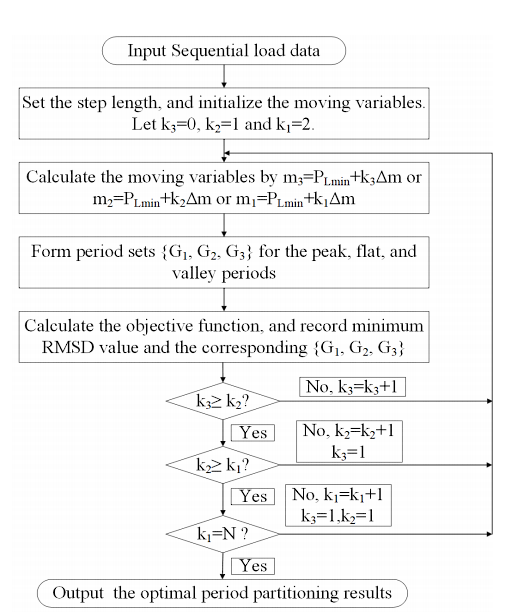
\includegraphics[scale=1]{fig3.jpg}
\caption{\textit{Flowchart of Peak Flat Valley period partition
}}
\end{figure}
\pagebreak
\section{Results}
The RTS and RBTS systems are used for the required data. The proposed method
was implemented in MATLAB software.
\subsection{Draw Load Curve}
The RTS and RBTS systems are used for the required data. The proposed method
was implemented in MATLAB software.\\
\begin{table}[!hbt]
\begin{center}
\caption{Sequential data}
\end{center}
\begin{tabular}{|c|c|c|}
\hline 
S.N. & Hour & Load in per  \\ 
 &  & unit \\ 
\hline 
1 & 12-1 am & 0.67 \\ 
\hline 
2 & 1-2 am & 0.63 \\ 
\hline 
3 & 2-3 am & 0.6 \\ 
\hline 
4 & 3-4 am & 0.59 \\ 
\hline 
5 & 4-5 am & 0.59 \\ 
\hline 
6 & 5-6 am & 0.6 \\ 
\hline 
7 & 6-7 am & 0.74 \\ 
\hline 
8 & 7-8 am & 0.86 \\ 
\hline 
9 & 8-9 am & 0.95 \\ 
\hline 
10 & 9-10 am & 0.96 \\ 
\hline 
11 & 10-11 am & 0.96 \\ 
\hline 
12 & 11-Noon & 0.95 \\ 
\hline 
\end{tabular}\hspace{0.2in} 
\begin{tabular}{|c|c|c|}
\hline 
S.N. & Hour & Load in per  \\ 
 &  & unit \\ 
\hline 
 13 & Noon-1 pm & 0.95 \\ 
 \hline 
 14 & 1-2 pm & 0.95 \\ 
 \hline 
 15 & 2-3 pm & 0.93 \\ 
 \hline 
 16 & 3-4 pm & 0.94 \\ 
 \hline 
 17 & 4-5 pm & 0.99 \\ 
 \hline 
 18 & 5-6 pm & 1 \\ 
 \hline 
 19 & 6-7 pm & 1 \\ 
 \hline 
 20 & 7-8 pm & 0.96 \\ 
 \hline 
 21 & 8-9 pm & 0.91 \\ 
 \hline 
 22 & 9-10 pm & 0.83 \\ 
 \hline 
 23 & 10-11 pm & 0.73 \\ 
 \hline 
 24 & 11-12 pm & 0.63 \\ 
 \hline   
\end{tabular} 
\end{table}
\vspace{1cm}
\begin{figure}[H]
\centering
\includegraphics[scale=1]{loadcurve.jpg}
\caption{\textit{Load Curve}}
\end{figure}
\pagebreak
\subsection{Period Partition}
The normalized sequential load data are provided from the RTS system to construct
the period partition. After drawing load curve, we used equal step length iteration
for peak, flat, valley period partition. The partitioned load curve is shown below:
\begin{figure}[H]
\centering
\includegraphics[scale=1]{curve2.jpg}
\caption{\textit{Partitioned load curve in peak, flat and valley period}}
\end{figure}
\pagebreak
\section{Conclusion}
We took the data from the RBTS and plotted the load curve before implementing
Time of Use Of electricity (TOU) and after drawing load curve, we used equal step
length iteration for peak, flat, valley period partition.

\pagebreak
\cite{yang2012game}
\bibliographystyle{ieeetran}
\section*{References}  
\bibliography{ref}
\end{document}
